\documentclass[11pt, a4paper]{article}

\usepackage[margin=2.5cm]{geometry}
\usepackage{amsmath}
\usepackage{amssymb}
\usepackage{graphicx}
\usepackage{hyperref}
\usepackage{parskip}

\title{\textbf{Interaction Networks}\\[0.4em]
       \large Robert Trifan}
\author{}
\date{}

\begin{document}

\maketitle
\thispagestyle{empty}
\vspace{-2em}

% ─────────────────────────────────────────────────────────────────────────────

\section{Introduction}

The $N$-body problem asks how a system of $N$ point masses evolves over time under mutual gravitational attraction.
For $N \geq 3$ no closed-form solution exists, so one must resort to numerical integration: compute all pairwise
forces, update velocities, advance positions, repeat.
Classical integrators (Euler, Leapfrog, Runge--Kutta) are accurate but scale as $\mathcal{O}(N^2)$ per step and
accumulate floating-point error over long horizons.

A complementary approach is to \emph{learn} the dynamics directly from simulated trajectories.
If a neural network can capture the underlying interaction law from data, it can be rolled out autoregressively
to predict future states without explicitly computing forces.
Such a model generalises across initial conditions and, because interactions are pairwise by nature, can
transfer to system sizes unseen during training.

Battaglia et al.\ (2016) introduced \textit{Interaction Networks} (INs)~\cite{battaglia2016interactionnetworkslearningobjects}, a graph neural network that models
a physical system as a directed graph: objects become nodes and directed pairs become edges.
A learned \emph{relational} MLP processes each edge (encoding how one object affects another) and produces an
interaction effect; a learned \emph{object} MLP then aggregates all incoming effects for each node and predicts
the object's next state.
The architecture is fully permutation-equivariant and compositional, making it a natural fit for $N$-body
dynamics.

This report describes a faithful re-implementation of the Interaction Network applied to the gravitational
$N$-body problem.
We reproduce the paper's model architecture (four-layer relational MLP with 150 hidden units, one-layer object MLP
with 100 hidden units), train on simulated three-body trajectories, and evaluate rollout accuracy and energy
conservation.
We also probe out-of-distribution generalisation by evaluating on five bodies after training on three.

% ─────────────────────────────────────────────────────────────────────────────

\section{Idea}

\subsection{Physical Setup}

We consider $N$ point masses in the two-dimensional plane.
Body $i$ has mass $m_i$, position $\mathbf{r}_i \in \mathbb{R}^2$, and velocity $\mathbf{v}_i \in \mathbb{R}^2$.
Here is what Newton woke up one morning and said:

\begin{equation}
       \mathbf{F}_{ij} = G \frac{m_i\,m_j}{|\mathbf{r}_j - \mathbf{r}_i|^2}\hat{\mathbf{r}}_{ji}
       \label{eq:force}
\end{equation}

This is the gravitational force exerted by body $j$ on body $i$, where $\hat{\mathbf{r}}_{ji}$ is the unit vector pointing from $i$ to $j$.

You can think of the magnitude of the force as:
\begin{equation}
    |\mathbf{F}_{ij}| = G \frac{m_i\,m_j}{|\mathbf{r}_j - \mathbf{r}_i|^2},
\end{equation}

and the direction as:
\begin{equation}
       \hat{\mathbf{r}}_{ji} = \frac{\mathbf{r}_j - \mathbf{r}_i}{|\mathbf{r}_j - \mathbf{r}_i|}.
\end{equation}

Hence the full vector form of the force is given by:

\begin{equation}
    \mathbf{F}_{ij} = G \frac{m_i\,m_j}{|\mathbf{r}_j - \mathbf{r}_i|^2} \cdot \frac{\mathbf{r}_j - \mathbf{r}_i}{|\mathbf{r}_j - \mathbf{r}_i|}
    = G \frac{m_i\,m_j\,(\mathbf{r}_j - \mathbf{r}_i)}{|\mathbf{r}_j - \mathbf{r}_i|^3}.
\end{equation}

Now we also now that $\mathbf{F} = m \mathbf{a}$, so the acceleration of body $i$ due to body $j$ is:
\begin{equation}
    \mathbf{a}_{ij} = \frac{\mathbf{F}_{ij}}{m_i} = G \frac{m_j\,(\mathbf{r}_j - \mathbf{r}_i)}{|\mathbf{r}_j - \mathbf{r}_i|^3}.
\end{equation}

note how $m_i$ cancels out, so the acceleration of body $i$ does not depend on its own mass, only on the masses of the other bodies and their relative positions.

\textit{remember: a feather and a hammer fall at the same rate in a vacuum, because their accelerations are independent of their masses!}

And the last piece of the puzzle is that the total acceleration of body $i$ is the sum of the accelerations due to all other bodies:
\begin{equation}
    \mathbf{a}_i = \sum_{j \neq i} \mathbf{a}_{ij} = G \sum_{j \neq i} \frac{m_j\,(\mathbf{r}_j - \mathbf{r}_i)}{|\mathbf{r}_j - \mathbf{r}_i|^3}.
    \label{eq:gravity}
\end{equation}

Ground-truth trajectories are generated with the \emph{velocity Verlet} integrator, which is second-order
accurate:

\begin{align}
    \mathbf{r}(t {+} \Delta t) &= \mathbf{r}(t) + \mathbf{v}(t)\,\Delta t
                                  + \tfrac{1}{2}\mathbf{a}(t)\,\Delta t^2, \\
    \mathbf{a}(t {+} \Delta t) &= \text{compute from } \mathbf{r}(t {+} \Delta t)
                                  \text{ via Eq.~\eqref{eq:gravity}}, \\
    \mathbf{v}(t {+} \Delta t) &= \mathbf{v}(t)
                                  + \tfrac{1}{2}\bigl[\mathbf{a}(t)
                                  + \mathbf{a}(t {+} \Delta t)\bigr]\Delta t.
\end{align}

Another important aspect of the physical is the preservation of energy.

We know that the kinetic energy of body $i$ is given by
\begin{equation}
       E_{\mathrm{kin}, i} = \frac{1}{2} m_i\,|\mathbf{v}_i|^2,
\end{equation}

and the potential energy of the system is given by
\begin{equation}
       E_{\mathrm{pot}} = -\, G\sum_{i < j} \frac{m_i\,m_j}{|\mathbf{r}_i - \mathbf{r}_j|}.
\end{equation}

Then the total mechanical energy becomes:

\begin{equation}
    E = \underbrace{\frac{1}{2}\sum_i m_i\,|\mathbf{v}_i|^2}_{E_{\mathrm{kin}}}
        \underbrace{-\, G\sum_{i < j}
          \frac{m_i\,m_j}{|\mathbf{r}_i - \mathbf{r}_j|}}_{E_{\mathrm{pot}}},
    \label{eq:energy}
\end{equation}

and should be conserved over time.

\subsection{Data Generation}


Masses are sampled as $m_i \sim \mathcal{U}(0.5,\,2.0)$, initial positions as
$\mathbf{r}_i \sim \mathcal{N}(\mathbf{0},\,3^2 I)$, and initial velocities as
$\mathbf{v}_i \sim \mathcal{N}(\mathbf{0},\,0.5^2 I)$, then shifted to the centre-of-mass frame
so that total momentum is zero.


\subsection{Graph Representation}

Formally the features for node $i$ at time $t$ are given by
\begin{equation}
    \mathbf{x}_i(t) = \bigl[\mathbf{r}_i(t),\;\mathbf{v}_i(t),\;m_i\bigr] \in \mathbb{R}^5.
\end{equation}

For edge features we use a scalar graph feature $\mathbf{g}_{ij} = [1]$ for all edges, so the network must learn to infer geometric relationships from the node features alone.

The label for node $i$ at time $t$ is the acceleration $\mathbf{a}_i(t)$ computed from the ground-truth trajectory via Eq.~\eqref{eq:gravity}.

We then build a directed graph with $N$ nodes and $N(N-1)$ edges, where each node has a 5-dimensional feature vector and each edge has a 1-dimensional feature vector.


\subsection{Interaction Network}

Since we defined information about bodies as node features and interactions as edge features, we can use a graph neural network to learn the dynamics.

The Interaction Network proposed by Battaglia et al.\ (2016)~\cite{battaglia2016interactionnetworkslearningobjects} describes how to enforce the message-passing structure of a GNN to match the physical structure of the $N$-body problem.

\paragraph{Relational model $f_R$.}
For each directed edge $j \to i$, a shared MLP computes an \emph{interaction effect} capturing the
influence of body $j$ on body $i$:

\begin{equation}
    \mathbf{e}_{ji} = f_R\!\bigl([\mathbf{x}_i,\;\mathbf{x}_j,\;\mathbf{g}_{ji}]\bigr) \in \mathbb{R}^{d_e}.
\end{equation}

The input is the concatenation of both endpoint feature vectors and the edge feature
($2\times 5 + 1 = 11$ dimensions); the output is a $d_e = 50$-dimensional effect vector.
$f_R$ consists of four hidden layers of 150 units each with ReLU activations.

\paragraph{Aggregation.}
The effects on node $i$ are summed over all incoming edges:

\begin{equation}
    \bar{\mathbf{e}}_i = \sum_{j \neq i} \mathbf{e}_{ji} \;\in\; \mathbb{R}^{d_e}.
\end{equation}

The sum-aggregation is permutation-invariant and preserves additivity of forces, matching the
structure of Eq.~\eqref{eq:gravity}.

\paragraph{Object model $f_O$.}
A second MLP takes the node's own features and its aggregated effect, and predicts the acceleration:

\begin{equation}
    \hat{\mathbf{a}}_i = f_O\!\bigl([\mathbf{x}_i,\;\bar{\mathbf{e}}_i]\bigr) \in \mathbb{R}^2,
\end{equation}

with input dimension $5 + 50 = 55$.
$f_O$ has one hidden layer of 100 units with ReLU activations.

Unlike the original paper (which predicts the next velocity) we predict acceleration directly.

\subsection{Training}

The network is trained to minimise the mean squared error between predicted and ground-truth accelerations:

\begin{equation}
    \mathcal{L} = \frac{1}{N\,T}\sum_{t=0}^{T}\sum_{i=1}^{N}
        \bigl|\hat{\mathbf{a}}_i(t) - \mathbf{a}_i(t)\bigr|^2.
\end{equation}

We use the Adam optimiser with initial learning rate $\eta = 10^{-3}$, halved every 25 epochs
($\gamma = 0.5$, StepLR).
Training uses 2\,000 simulated three-body trajectories of 100 time steps ($\Delta t = 0.01$), yielding
roughly 200\,000 labelled graph snapshots.

\subsection{Autoregressive Rollout}

At inference time the model is unrolled autoregressively.
Given state $(\mathbf{r}(t),\,\mathbf{v}(t))$, the graph is constructed, the network predicts
$\hat{\mathbf{a}}(t)$, and the state is advanced via \emph{Euler} integration:

\begin{align}
    \mathbf{v}(t {+} \Delta t) &= \mathbf{v}(t) + \hat{\mathbf{a}}(t)\,\Delta t, \\
    \mathbf{r}(t {+} \Delta t) &= \mathbf{r}(t) + \mathbf{v}(t {+} \Delta t)\,\Delta t.
\end{align}

And we can evaluate the rollout by comparing the predicted trajectory to the ground-truth trajectory generated by the velocity Verlet integrator.

% ─────────────────────────────────────────────────────────────────────────────

\section{Results}

We evaluate model performance using the following metrics:

\begin{itemize}
    \item \textbf{Rollout mean squared error (MSE):} the mean squared error between the predicted and ground-truth trajectories over the rollout horizon.
    \item \textbf{Constant-velocity baseline:} a baseline rollout where each body keeps its initial velocity, used to check whether the learned model improves over a simple no-force predictor.
    \item \textbf{Energy drift:} the total mechanical energy computed from the predicted trajectory and compared against the initial energy of the system.
\end{itemize}

The best run used the paper-style architecture with a four-layer relational MLP of 150 hidden units,
a 50-dimensional effect vector, and a one-hidden-layer object MLP of 100 hidden units.
It was trained on 2\,000 three-body simulations for 200 epochs with learning rate $10^{-3}$ and batch size 256.

\begin{table}[h]
    \centering
    \begin{tabular}{ll}
        \hline
        \textbf{Quantity} & \textbf{Value} \\
        \hline
        Best validation acceleration MSE & $6.21371 \times 10^{-3}$ \\
        Best epoch & 197 \\
        Number of trainable parameters & 83\,102 \\
        Training time & 1\,184.8 seconds ($\approx 19.7$ minutes) \\
        \hline
    \end{tabular}
    \caption{Best training results for the three-body Interaction Network run.}
    \label{tab:best-results}
\end{table}

\begin{figure}[h]
    \centering
    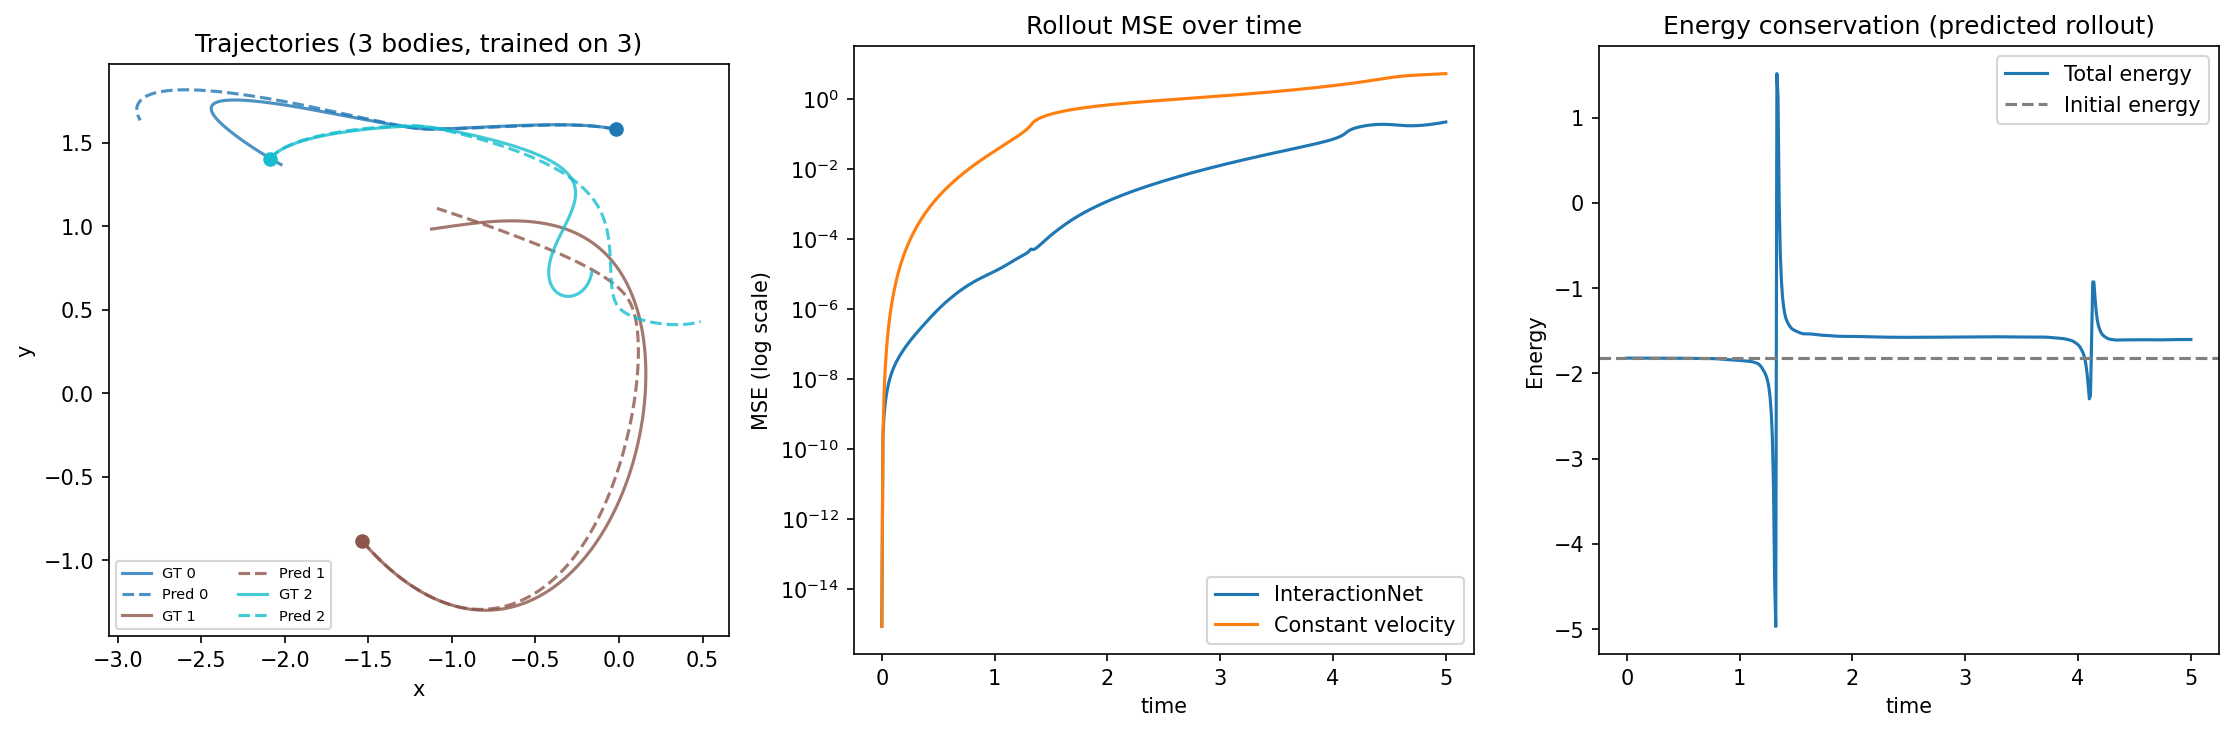
\includegraphics[width=\textwidth]{images/eval_3body.png}

    \small Three-body rollout

    \vspace{1em}

    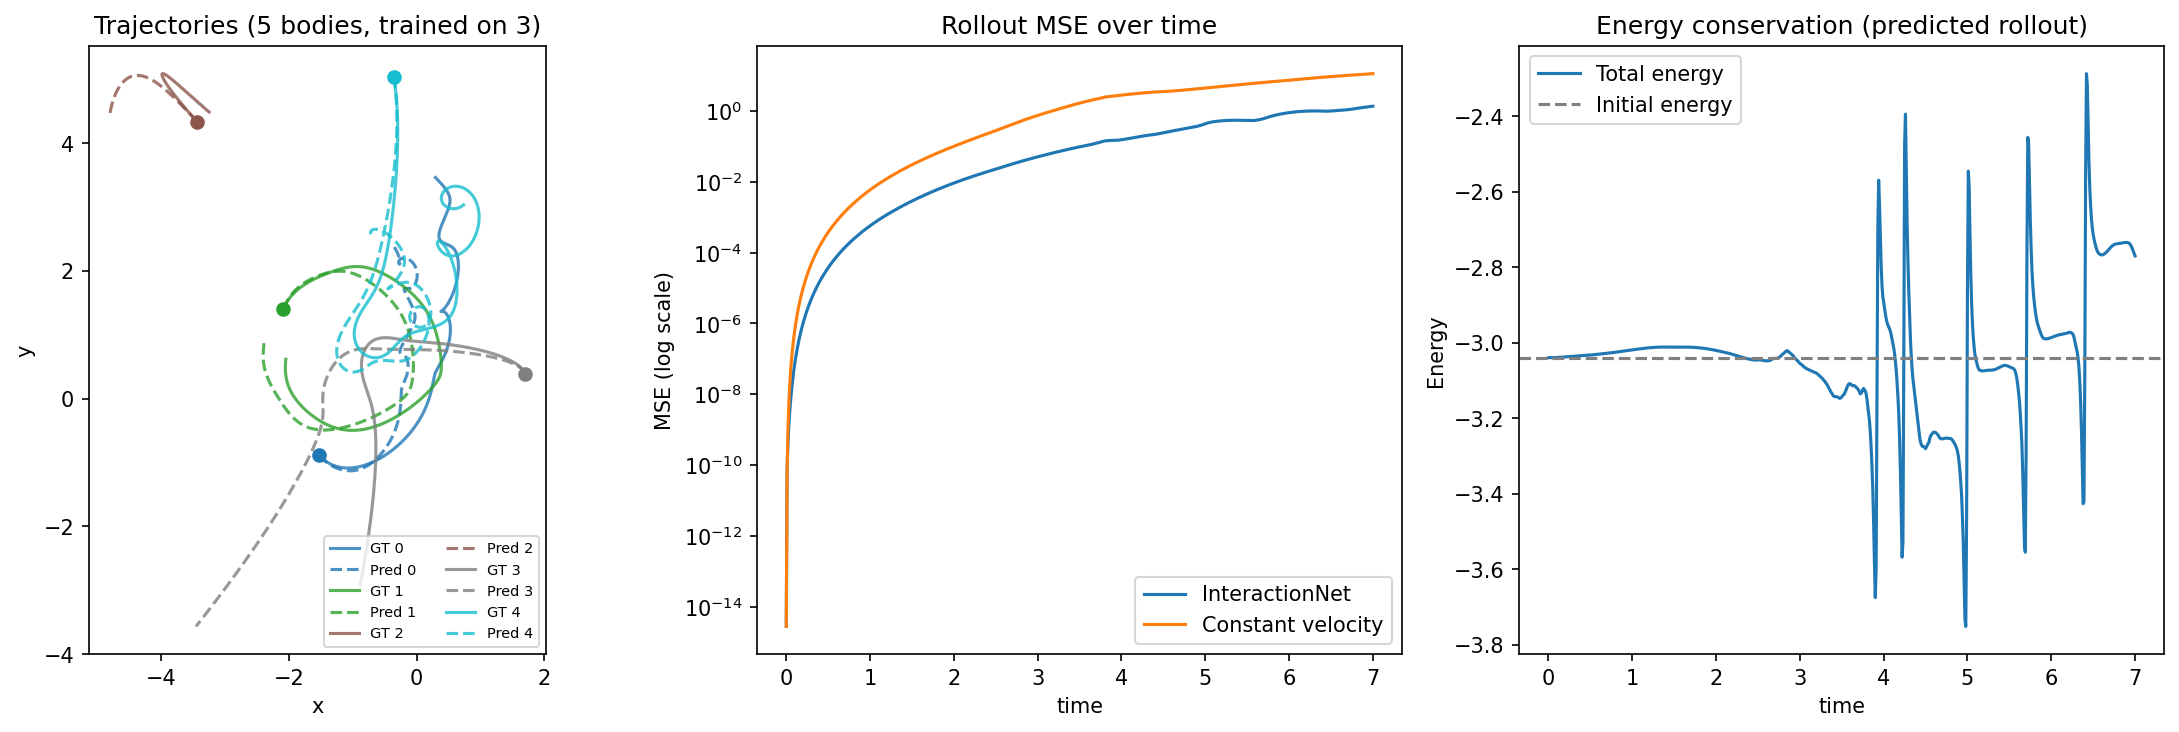
\includegraphics[width=\textwidth]{images/eval_5body.png}

    \small Five-body rollout

    \caption{Evaluation rollouts for the trained three-body model on in-distribution three-body dynamics and out-of-distribution five-body dynamics.}
    \label{fig:evaluation-rollouts}
\end{figure}


\section{Conclusion}

The Interaction Network successfully learned physical dynamics from data, achieving a low acceleration MSE and producing accurate rollouts that closely match the ground-truth trajectories.
One aspect worth exploring further is how to model what happens when two bodies get very close to each other, since the root cause of large errors starts from close encounters where the force magnitude and energy change rapidly.
The model's ability to generalise to five-body dynamics after training on three-body dynamics is promising, demonstrating that \textit{Graph Neural Networks} can capture the underlying interaction structure and transfer to larger systems.



\begin{thebibliography}{1}

\bibitem{battaglia2016interactionnetworkslearningobjects}
Peter W. Battaglia, Razvan Pascanu, Matthew Lai, Danilo Rezende, and Koray Kavukcuoglu.
\newblock \textit{Interaction Networks for Learning about Objects, Relations and Physics}.
\newblock arXiv:1612.00222, 2016.
\newblock \url{https://arxiv.org/abs/1612.00222}.

\end{thebibliography}

\end{document}
